\chapter{Updates}
\section{Einleitung}
Updates gehören zu den effektivsten Möglichkeiten, sich gegen Angreifer zu schützen.
Für Angreifer ist es ein goldenes Los Software zu entdecken, welche nicht aktualisiert wurde und tendenziell sogar ein \acrfull{cve}\footnote{Link: https://www.cve.org/} dazu existiert.\\

Daher ist es wichtig, möglichst zeitnah aktuelle Updates zu installieren.
Viele Softwarehersteller bieten eine automatische Updatefunktion, welche die neusten Updates direkt installiert.

\section{Windows Updates}
Windows Updates können direkt in den Systemeinstellungen heruntergeladen und installiert werden.
Dies muss jedoch standardmässig von den Benutzern gemacht werden.
Diese Updates können über die Group Policy erzwungen werden, damit sichergestellt werden kann, dass die System immer auf aktuellen Stand sind.\\

Wichtige Anmerkung:
\begin{lstlisting}
Bei kritischen Systemen muss immer zuerst überprüft werden, ob alle Funktionen nach dem Update noch funktionieren.
\end{lstlisting}

\subsection{\acrshort{gpo} für Clients}
Falls kritische Clients vorhanden sind, sollte \acrfull{wsus} verwendet werden. Siehe Kapitel \hyperref[subsec:wsus]{WSUS}\\

Im Group Policy Management muss eine neue Group Policy erstellt werden, welche mit der \acrshort{ou} verknüpft ist, die alle Windows Geräte enthält.
\begin{figure}[H]
    \centering
    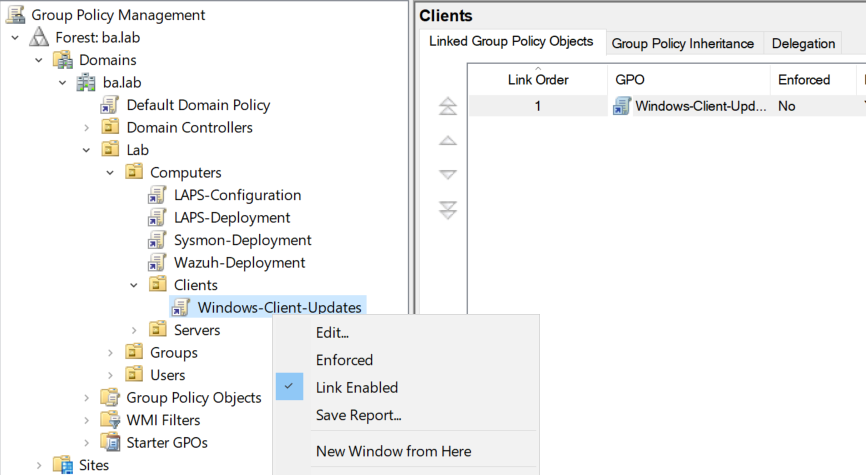
\includegraphics[width=0.7\linewidth]{../img/Updates/edit-gpo-clinets.png}
    \caption{Neue \acrshort{gpo} für Windows Client Updates}
\end{figure}

Mit \textbf{Rechtsklick $\rightarrow$ Edit} kann die neue Group Policy bearbeitet werden.
Unter \textbf{Computer Configuration $\rightarrow$ Policies $\rightarrow$ Administrative Templates $\rightarrow$ Windows Components $\rightarrow$ Windows Update} findet man alle Policies bezüglich Windows Updates.
Für Clients werden folgende Policies eingerichtet:

\begin{minipage}{0.5\linewidth}
    \begin{figure}[H]
        \centering
        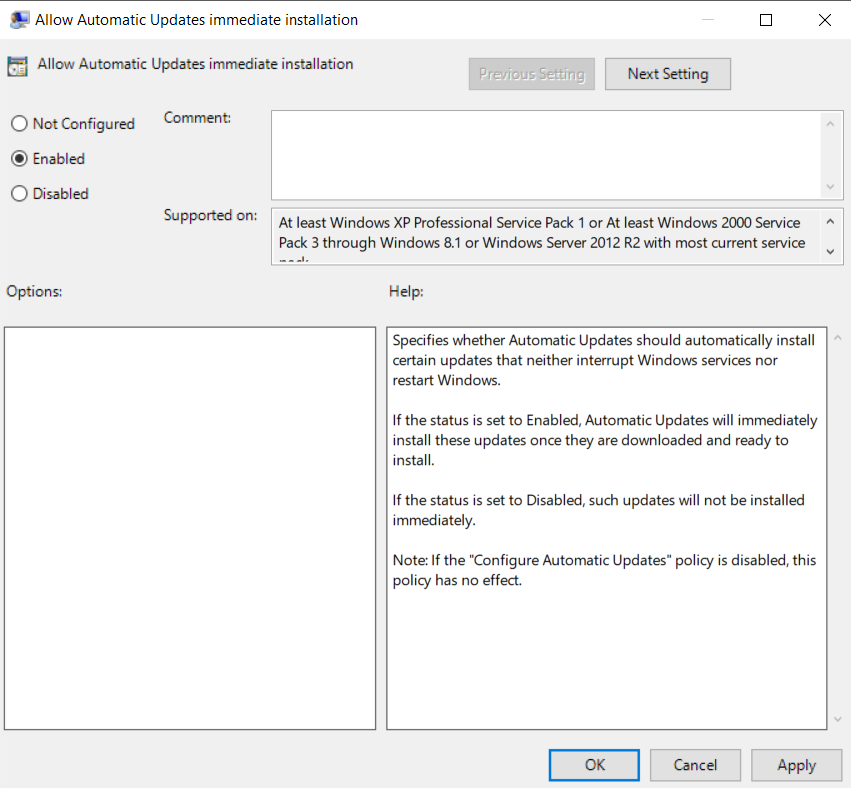
\includegraphics[width=\linewidth]{../img/Updates/client-allow-immediate-updates.png}
        \caption{\acrshort{gpo} Client Updates 1}
    \end{figure}
\end{minipage}
\begin{minipage}{0.5\linewidth}
    \begin{figure}[H]
        \centering
        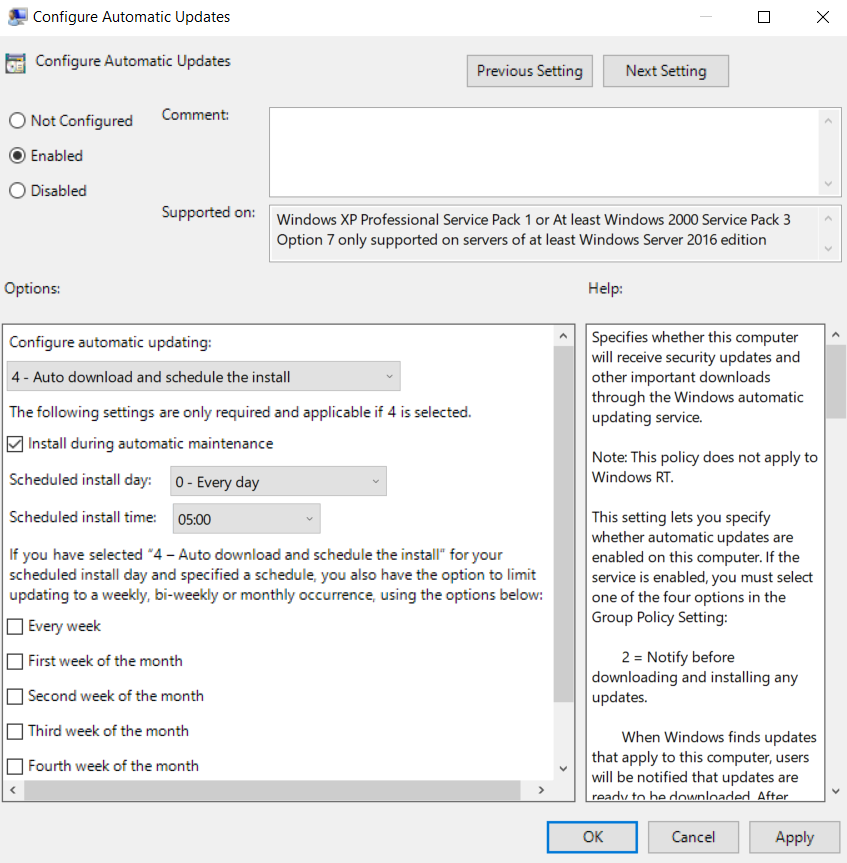
\includegraphics[width=\linewidth]{../img/Updates/client-configure-automatic-updates.png}
        \caption{\acrshort{gpo} Client Updates 2}
    \end{figure}
\end{minipage}\\
\begin{minipage}{0.5\linewidth}
    \begin{figure}[H]
        \centering
        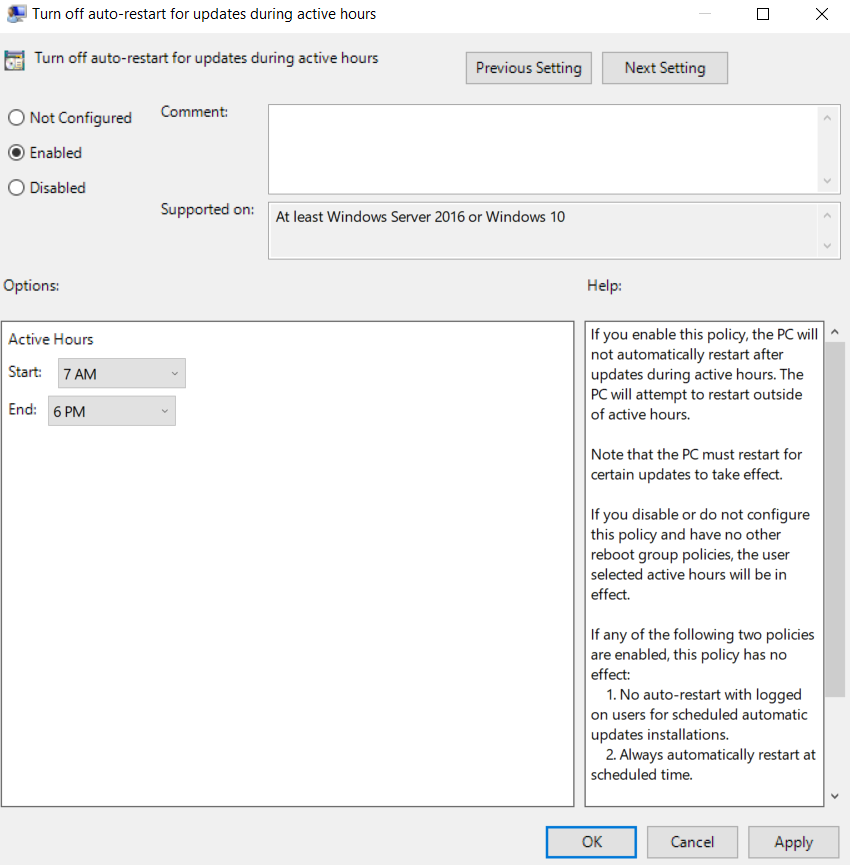
\includegraphics[width=\linewidth]{../img/Updates/client-auto-restart-during-working-hours.png}
        \caption{\acrshort{gpo} Client Updates 3}
    \end{figure}
\end{minipage}
\begin{minipage}{0.5\linewidth}
    \begin{figure}[H]
        \centering
        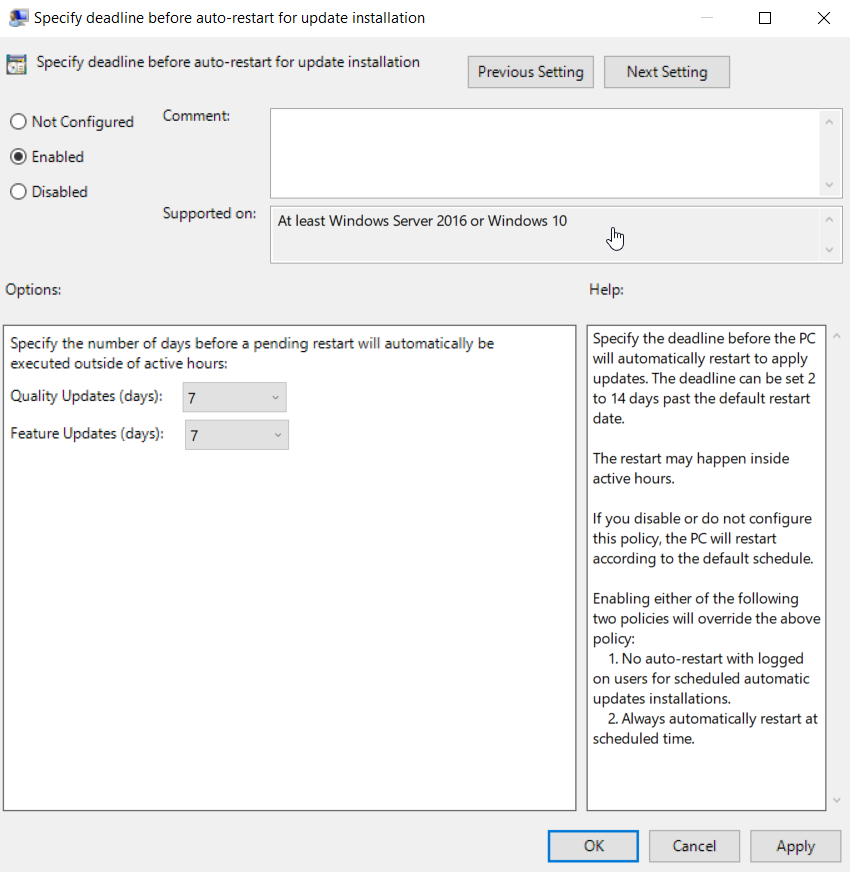
\includegraphics[width=\linewidth]{../img/Updates/client-force-restart-deadline.png}
        \caption{\acrshort{gpo} Client Updates 4}
    \end{figure}
\end{minipage}\\

Mit diesen Einstellungen werden die Updates am Morgen, um 05:00 Uhr,  heruntergeladen und installiert.
Die Benutzer müssen spätestens nach 7 Tagen ihre Computer neu starten.
Ausserdem werden die Computer nur ausserhalb der definierten Arbeitszeit automatisch neu gestartet.\\

Diese Einstellungen sollen nicht strikt übernommen werden, sondern den Bedürfnissen des Betriebs angepasst werden.
Wichtig ist jedoch, dass die Updates automatisch installiert werden und das die Computer nach Updates neugestartet werden müssen.

\subsection{\acrshort{gpo} für Server}
Falls kritische Server vorhanden sind, sollte \acrfull{wsus} verwendet werden. Siehe Kapitel \hyperref[subsec:wsus]{WSUS}\\

Updates für Server sollten installiert werden, wenn Sie nicht in Verwendung sind, da sie für kurze Zeit nicht verfügbar sein werden.
Daher ist die Group Policy für Server anderst als für Clients.
Für Server die 24/7 verwendet werden, muss ein ``Maintenance Window'' gesetzt und alle Benutzer informiert werden.\\

Im Group Policy Management muss eine neue Group Policy erstellt werden, welche mit der \acrshort{ou} verknüpft ist, die alle Windows Geräte enthält.
\begin{figure}[H]
    \centering
    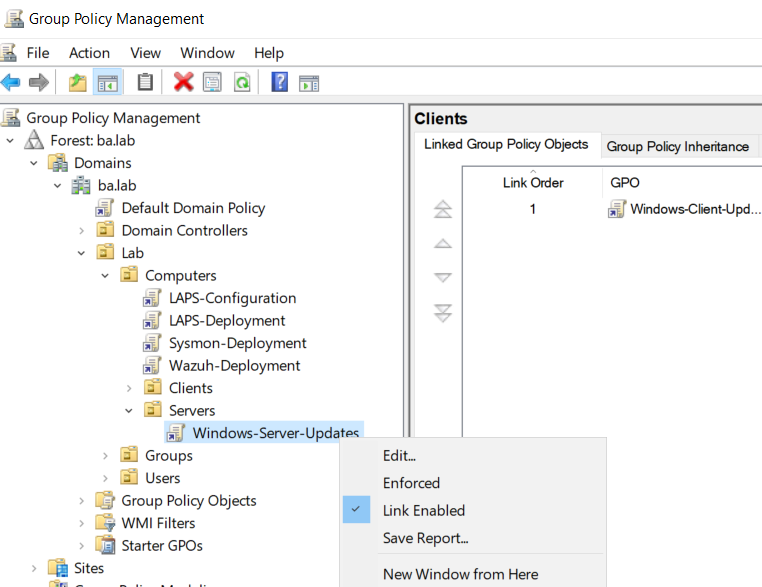
\includegraphics[width=0.7\linewidth]{../img/Updates/edit-gpo-server.png}
    \caption{Neue \acrshort{gpo} für Windows Server Updates}
\end{figure}

Mit \textbf{Rechtsklick $\rightarrow$ Edit} kann die neue Group Policy bearbeitet werden.
Unter \textbf{Computer Configuration $\rightarrow$ Policies $\rightarrow$ Administrative Templates $\rightarrow$ Windows Components $\rightarrow$ Windows Update} findet man alle Policies bezüglich Windows Updates.
Für Server werden folgende Policies eingerichtet:

\begin{minipage}{0.5\linewidth}
    \begin{figure}[H]
        \centering
        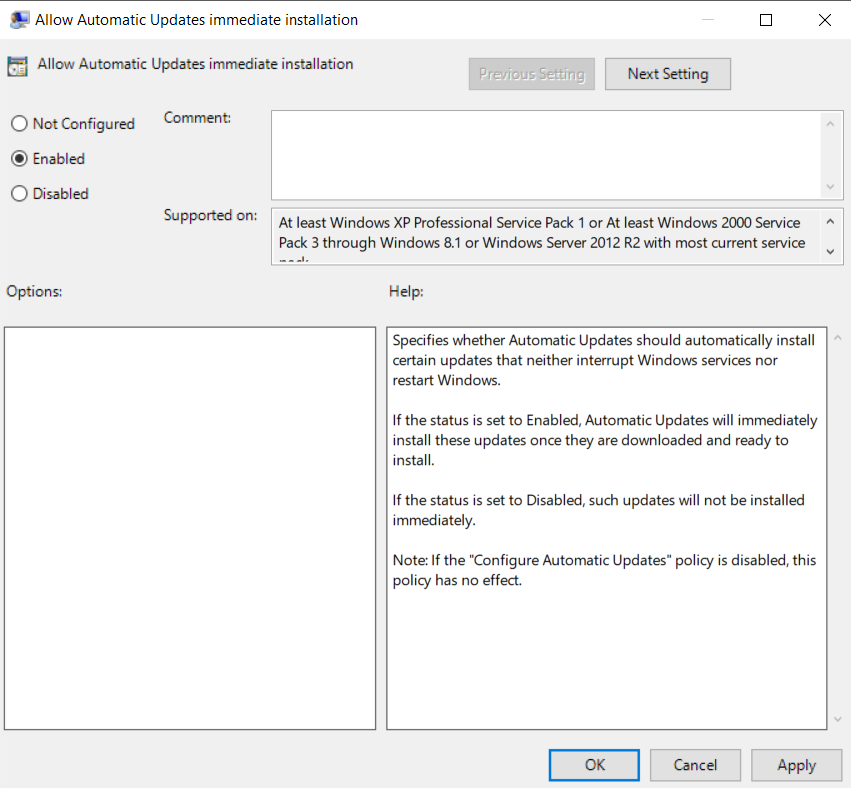
\includegraphics[width=\linewidth]{../img/Updates/client-allow-immediate-updates.png}
        \caption{\acrshort{gpo} Server Updates 1}
    \end{figure}
\end{minipage}
\begin{minipage}{0.5\linewidth}
    \begin{figure}[H]
        \centering
        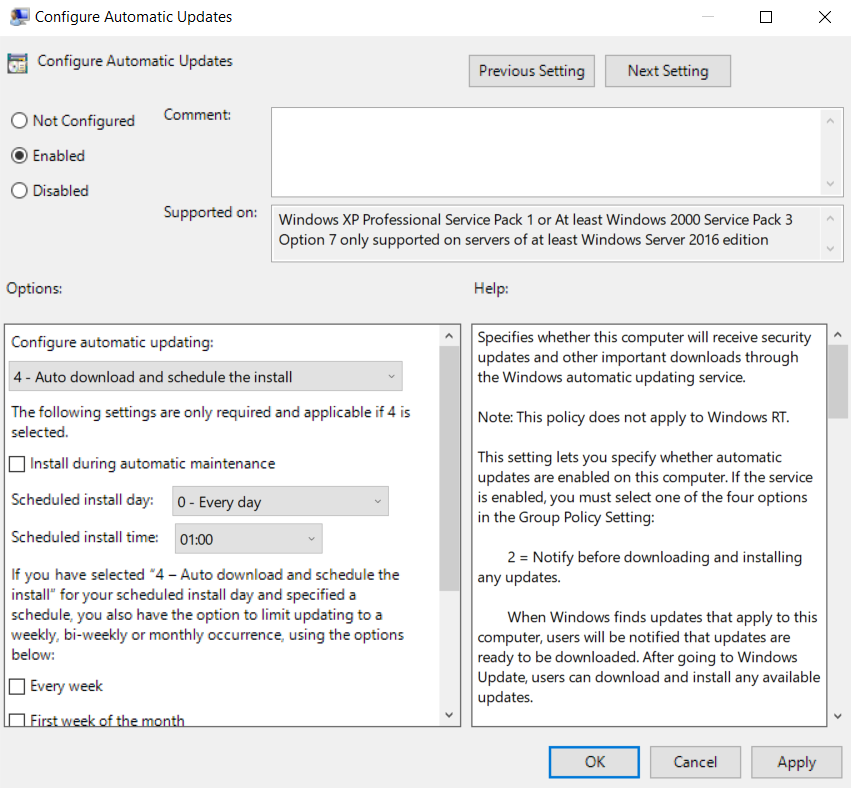
\includegraphics[width=\linewidth]{../img/Updates/server-configure-automatic-updates.png}
        \caption{\acrshort{gpo} Server Updates 2}
    \end{figure}
\end{minipage}\\
\begin{minipage}{0.5\linewidth}
    \begin{figure}[H]
        \centering
        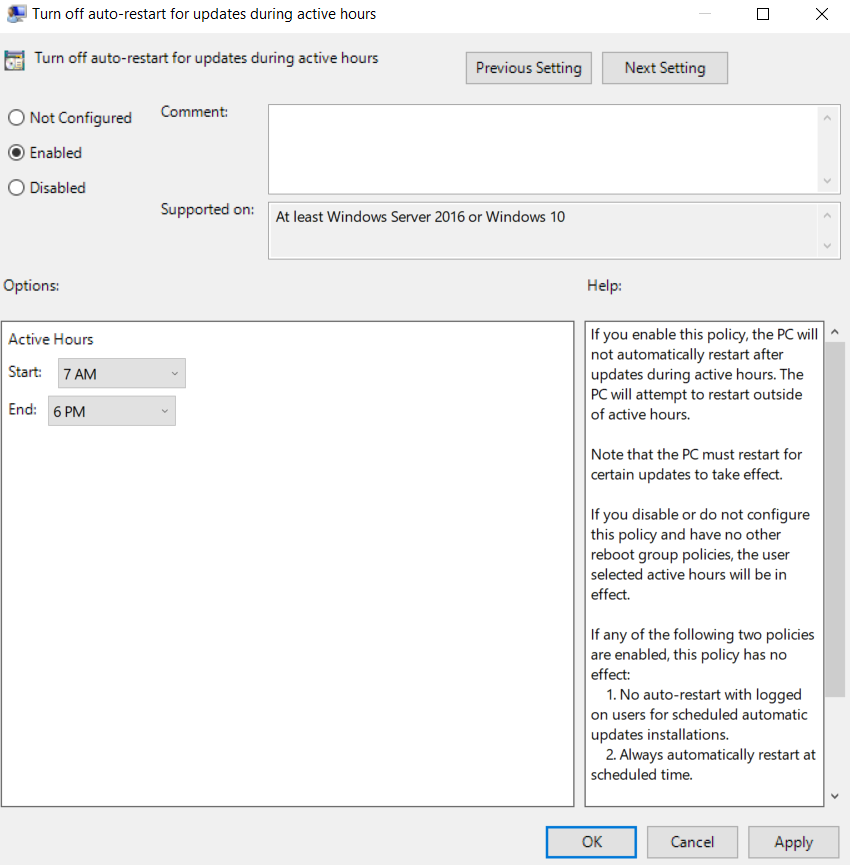
\includegraphics[width=\linewidth]{../img/Updates/client-auto-restart-during-working-hours.png}
        \caption{\acrshort{gpo} Server Updates 3}
    \end{figure}
\end{minipage}
\begin{minipage}{0.5\linewidth}
    \begin{figure}[H]
        \centering
        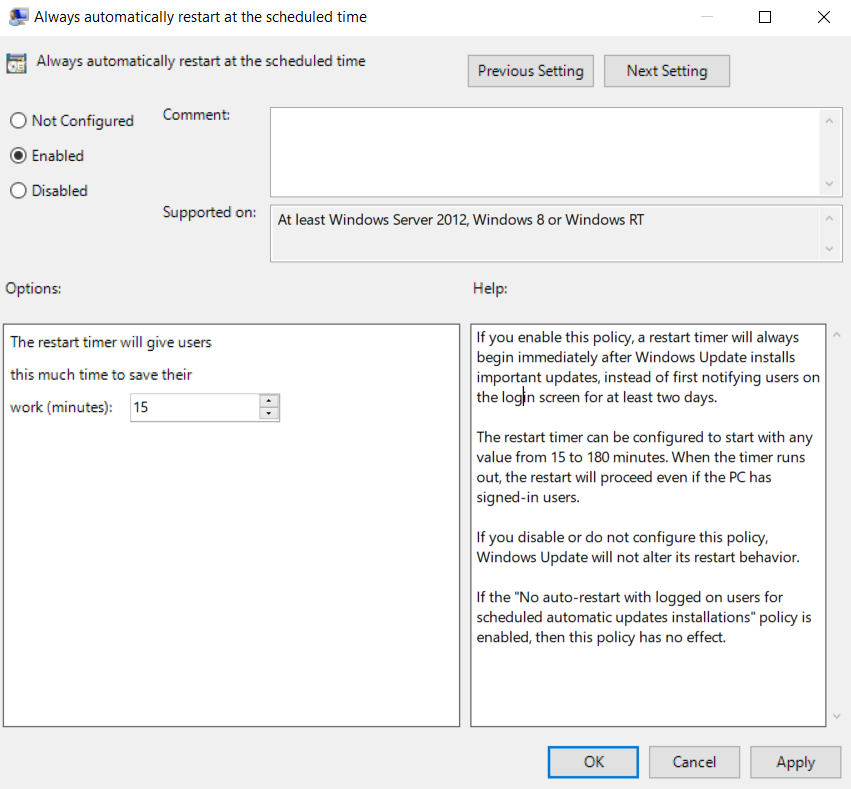
\includegraphics[width=\linewidth]{../img/Updates/server-automatic-restart.png}
        \caption{\acrshort{gpo} Server Updates 4}
    \end{figure}
\end{minipage}\\

Die Updates werden auf den Servern in der Nacht, um 01:00 Uhr, installiert und die Server anschliessend neu gestartet.
Für kritische Server sollten die Updates zuerst getestet werden und manuell installiert werden.

\subsection{\acrfull{wsus}}\label{subsec:wsus}
Falls neben den regulären auch kritische Systeme vorhanden sind, lohnt es sich einen WSUS Server einzurichten.
Dieser bietet die Möglichkeit, Computer und Server in Gruppen einzuteilen und genauer zu definieren, welche Gruppe wann welche Updates erhält.
WSUS ist eine Serverrolle auf Windows Server und kann über den Server Manager installiert werden.\\

In diesem Guide wird nicht genauer auf die Verwendung von WSUS eingegangen.
Microsoft bietet gute \href{https://docs.microsoft.com/de-de/windows-server/administration/windows-server-update-services/get-started/windows-server-update-services-wsus}{Anleitungen}\footnote{Link: https://docs.microsoft.com/de-de/windows-server/administration/windows-server-update-services/get-started/windows-server-update-services-wsus}, wie WSUS installiert und eingerichtet werden kann.


\section{Updates weiterer Software}
Für weitere Software, welche nicht zentral verwaltet werden kann, sollte ein Update-Konzept erstellt werden.
Neue Updates sollten in einem festgelegten Rythmus auf allen betroffenen Systemen installiert werden.